\title{Golf Practice Animation Report}
\author{}
\documentclass[a4paper,11pt]{article}
\usepackage[utf8]{inputenc}
\usepackage{pdfpages}
\usepackage{amssymb}
\usepackage{amsmath}
\usepackage{float}
\usepackage{siunitx}        % Provides the \SI{}{} and \si{} command for typesetting SI units
\usepackage{graphicx}       % Required for the inclusion of images
\usepackage[shortlabels]{enumitem}
\usepackage[T1]{fontenc}
\usepackage{geometry}
\geometry{a4paper, total={6in, 8in}, margin=25mm} %margins
\usepackage{hyperref}
\hypersetup{colorlinks=true,linkcolor=black, citecolor=black}
\usepackage{tocloft}
\usepackage{lastpage}
\usepackage{fancyhdr}
\usepackage{subfig}
\pagestyle{fancy}
\renewcommand{\headrulewidth}{0pt}
\fancyhead{}
\lfoot{\fontsize{9}{9} \selectfont EMI Capstone Final Report (ENGR90038)\\ Copyright © \theauthor, 2020}
\cfoot{\fontsize{9}{9} \selectfont \today}
\rfoot{\fontsize{9}{9} \selectfont Page \thepage \ of \pageref{LastPage}}


\makeatletter

\date{\today}               % Date for the report
\let\thetitle\@title        % Document title saved in command
\let\theauthor\@author      % Document author saved in command

\makeatletter
\g@addto@macro\@floatboxreset\centering
\makeatother
\renewcommand{\cftsecleader}{\cftdotfill{\cftdotsep}}

\usepackage{fontspec}
% Times New Roman
\setromanfont[
BoldFont=timesbd.ttf,
ItalicFont=timesi.ttf,
BoldItalicFont=timesbi.ttf,
]{times.ttf}
% Arial
\setsansfont[
BoldFont=arialbd.ttf,
ItalicFont=ariali.ttf,
BoldItalicFont=arialbi.ttf
]{arial.ttf}

\setlength{\parindent}{0pt}
\setlength{\parskip}{6pt}
\usepackage{changepage}

\usepackage{titlesec}

\titleformat*{\section}{\Large\bfseries\sffamily}
\titleformat*{\subsection}{\large\bfseries\sffamily}
\titleformat*{\subsubsection}{\normalsize\bfseries\sffamily}

\usepackage[]{xcolor}
\definecolor{melblue}{RGB}{31, 54, 90}
\definecolor{hrule}{RGB}{89, 128, 184}

\usepackage[style=apa]{biblatex}
\addbibresource{ref.bib}

\begin{document}

\begin{center}
    
\includegraphics[width=3cm, height=3cm]{icon.png}
    \\[1cm]
    \fontsize{16}{16}\sffamily\bfseries\textcolor{melblue}{Golf Practice Animation}
    \vspace{5pt}
    \textcolor{hrule}\hrule
    \vspace{20pt}
    \color{black}\fontsize{11}{11}
    \bfseries\sffamily Qionghui Cai
    \\
    \mdseries\rmfamily 950415, qionghuic@student.unimelb.edu.au
    \\[1cm]
    \bfseries\sffamily Yifan Xing
    \\
    \mdseries\rmfamily 947930, yifxing@student.unimelb.edu.au
    \\[1cm]
    \bfseries\sffamily Zijie Yang
    \\
    \mdseries\rmfamily 825694, zijiey@student.unimelb.edu.au
    \\[1cm]

\end{center}

\begin{adjustwidth*}{1cm}{1cm}
\textbf{\textit{Executive Summary:}} \textit{This guide provides formatting instructions for your Final Report. When you write reports in industry you will most likely have a “house” style that must be followed. This report provides a “house” style that you must follow. An executive summary of no more than 300 words should be provided here in the format given. The words ‘Executive Summary’ should be made bold as shown. Simply replace this italics text with your Executive Summary, which should be formatted as a single (continuous) paragraph, contain no in-text citations or make any reference to figures and tables. As a minimum, authors should use the executive summary to clearly identify the following: (i) the topic of the research presented; (ii) why this topic is of relevance to the wider community; and (iii) the extent to which the report establishes a novel view or presents new data, analyses or findings and/or conveys a useful message not already prevalent in peer-reviewed literature on the topic. Leave one line (space) free between this section and the next.}
\end{adjustwidth*}
\vspace{\fill}

\thispagestyle{empty}
\newpage

\tableofcontents{\protect\thispagestyle{empty}}
\pagestyle{fancy}
\clearpage
\setcounter{page}{1}
\newpage



\section{Introduction}


\subsection{Test}
\subsubsection{Test}
test \textcite{dirac} test
test


\section{Literature Review}


\section{Hardware design}


\subsection{radar selection}
\subsection{amplifying filter circuit design}
\subsection{power supply circuit design}
\subsection{offset circuit design}

\newpage
\section{Prediction Model}
\subsection{Kinematic Model}
The flying golf ball is mainly affected by gravity, drag force from air resistance, buoyancy and magnus force, showed as figure. Among them, the strength of magnus force is related to the rotational speed, difficult to be measured. The magnitude of the buoyancy is two orders smaller than the gravity and drag force, which is usually can be neglected.
Gravity is caused by the attraction force of the earth, always with a direction going straight down. It can be defined by the equation:
\begin{align}
F_{g}=m g
\end{align}
When the golf is flying, its surrounding air exerts a drag on it to push it back, opposite to the direction of velocity. This drag force has a nonlinear relationship with the velocity.
\begin{align}
\vec{F}_{d}=-\frac{1}{2} C_{D} \rho A v^{2} \frac{\vec{v}}{|v|}
\end{align}
where C$_D$ is the drag coefficient, with a common value 0.4. $\rho$ is air density, equaling to 1.23kg/m $^3$. A is the cross section area of the ball,related to the radius of golf ball. Typically, the radius of golf is


\subsection{Velocity Calculation}
Let’s assume the flying object is R distance away from the receiving antennas. The numbers of wavelength corresponding to the distance back and forth is:
\begin{align}
n=\frac{2 R}{\lambda}    
\end{align}
wavelength is define as:
\begin{align}
\lambda=\frac{c}{f_{t}}
\end{align}
Where $c=3 \times 10^{8} ; f_{t}=24 G H z$in this project\\
Since a wavelength means a 2 $\pi$ phase transformation. The total phase change is:
\begin{align}
\phi=2 \pi\left(\frac{2 R}{\lambda}\right)=4 \pi R / \lambda
\end{align}
The angular frequency refers to the rate of phase change when distance R varies over time. That is:
\begin{align}
\omega_{d}=\frac{d \phi}{d t}=\frac{4 \pi}{\lambda} \frac{d R}{d t}=\frac{4 \pi V_{r}}{\lambda}=2 \pi f_{d}
\end{align}
where $V_{r}=d R / d t$ and $f_{d}$ is Doppler frequency.\\
Rearrange the above equation, we get:
\begin{align}
V_{r}=\frac{\lambda}{2} f_{d}=V \cos \Theta
\end{align}
The velocity we get above is the radial velocity with angle $/theta$ with respect to the ground. Since the most critical value we need is the initial velocity infinitely approaching the swing point. The angle $/theta$ can be considered as 0 degree. That is:
\begin{align}
V=\frac{\lambda}{2} f_{d}
\end{align}


\subsection{Angle Calculation}
The main method we used to get angle is phase comparison method. Showed as figure , two antennas in the same direction separated by d meter receive the same ratio signal transmitting through directive antenna. The return signals received have same amplitude but different phases. Take the earth ground as the horizontal line. Assume the flying direction of the target is $\theta$, the phase difference should be:
\begin{align}
\begin{split}
\Delta \phi=2 \pi \frac{d}{\lambda} \sin \theta\\
\theta=\arcsin \frac{\lambda \Delta \phi}{2 \pi d}
\end{split}
\end{align}
In this project, a special 3-dimensions coordinate system with three axes is adopted. X axis represents the left and right space. Z axis represents the front and back space. Y axis represents the up and down space. In this way, the position of the flying ball will involve two angles. One is called azimuth related to x and z axes. The other one is called elevation, the angle between the golf and the horizon. Showed as figure.


\subsection{Kinematic Model}
Velocity decompose into x,y and z axis:
\begin{align}
\begin{split}
    V_{x}&=V \cdot \cos \alpha \cdot \cos \theta\\
    V_{z}&=V \cdot \cos \alpha \cdot \sin \theta\\
    V_{y}&=V \cdot \sin \theta    
\end{split}
\end{align}
According to the kinematic model and Newton’s second law:\\
x axis:
when $v_{x 0}>0$
\begin{align}
    m \frac{\partial^{2} x}{\partial t^{2}}=-k\left(\frac{\partial x}{\partial t}\right)^{2}
\end{align}
The initial conditions of above equations are:
\begin{align}
    \left.x\right|_{t=0}=0,\ \left.v_{x}\right|_{t=0}=v_{0 x}
\end{align}
where
\begin{align*}
      m &-- the mass of golf,kg\\
      g &-- gravitational acceleration, 9.8m/s^2\\
      t &-- flying time, s\\
      k &-- friction coefficient between the golf and air\\
      x,y,z &--the trajectory coordinate of golf at t moment   
\end{align*}



\newpage
\section{Software design}
The back-end software of the project runs on a single board computer (Raspberry Pi 4). The front-end software of the project is designed to run on mainstream operating systems or platforms such as iOS, Android, Windows and macOS. Through the modular design, each module can be developed using the most suitable programming language to achieve the best development efficiency and maintainability. About three thousand lines of code including C, python and C\# constitute the software part of the project. The software design of this project needs to have the following functions: 
\begin{itemize}[noitemsep,topsep=0pt]
   \item Read ADC data through SPI protocol
   \item Analyse the radar data to get the launch speed and angle of the ball
   \item Compute the flight trajectory of the golf ball from the launch speed and angle
   \item Display flight trajectory on any supported front-end device
\end{itemize}
   
Ideally, the back-end system is designed to run automatically without user action after the power is turned on. The front-end system needs to have an easy-to-use graphic user interface for users to operate.

\subsection{Software Architecture}
The back-end server of this project is based on Raspberry Pi OS (formerly Raspbian), which is a Debian derivative for Raspberry Pi. The stability and large open-source community of Debian bring convenience to the project development. The front-end application is based on the Unity 3D engine. This engine was selected because of its cross-platform portability.
\\
Due to the impact of the epidemic, the communication and cooperation of the project team are affected by the level 3 restrictions and time difference. Through object-oriented programming, different modules can be assigned to different team members. By deploying Git for version control, and the use of low coupling and high cohesion program design, the impact of the epidemic on teamwork is minimised.
\begin{figure}[H]
    \centering
    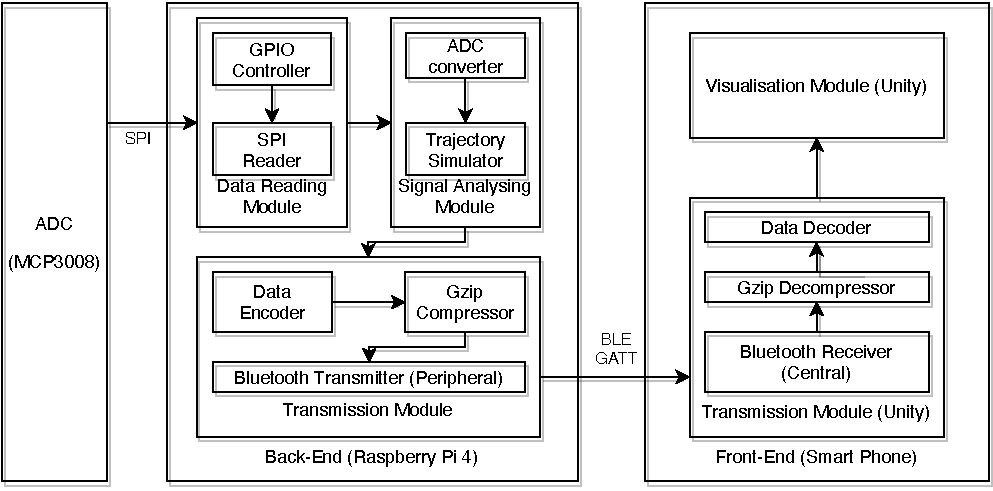
\includegraphics[width=\textwidth]{figure/Software.pdf}
    \caption{Software Architecture Diagram}
    \label{fig:software_diagram}
\end{figure}
The software architecture diagram is shown in Figure \ref{fig:software_diagram}. The back-end server contains three modules. The data reading module is responsible for operating the ADC. The signal processing module is used to compute the flight trajectory from the radar signal. The transmission module is responsible for communicating with the front-end device. The front-end application contains two modules. The transmission module communicates with the back-end server, and the visualisation module displays the flight trajectory on the user interface
\subsection{ADC Reading}
\subsubsection{SPI protocol}

\subsection{Signal Processing}
琼慧写
\subsection{Trajectory Simulation}
琼慧写
\subsection{Wireless Communication Solution}

\subsubsection{Communication Protocol selection}

\subsubsection{Bluetooth Communication module}


\subsubsection{Data Compression}




\subsection{Visualization}
\subsubsection{Platform selection}





\section{Results \& Analysis}


\section{Discussion}


\section{Conclusions and Recommendations}


\section{Acknowledgements }


\section{References}


\printbibliography[heading=none]


\section{Appendices/Supplementary Material}


\end{document}
